\chapter{Stato dell'Arte}
\section{Sistemi Ferroviari e Ferrotramviari}
Il concetto di \emph{treno} come comunemente percepito nasce con l'inizio della Rivoluzione Industriale, avvenuta tra il \emph{XVIII} e il \emph{XIX} secolo, a seguito della quale l'avvento della macchina a vapore ha permesso all'umanit\`a di disporre di fonti di energia sufficienti a fare evolvere i primi rudimentali trasporti su binario negli odierni sistemi ferroviari.\\*
\noindent\`E possibile schematizzare un Sistema Ferroviario, o Ferrotramviario, come un veicolo, il treno, vincolato a muoversi attraverso una propulsione, elettrica o a combustibile, lungo una traccia fissa, il binario.\\*
Queste caratteristiche accomunano qualsiasi sistema di trasporto ferroviario o ferrotramviario a prescindere dalla sua scala in termini di veicoli transitanti ed estensione geografica. Ci\'o che invece differenzia un Sistema Ferroviario da un Sistema Ferrotramviario sono:
\begin{itemize}
	\item Le caratteristiche fisiche del treno, come lunghezza e massa;
	\item Le caratteristiche geografiche dell'ambiente operativo;
	\item Gli scopi del trasporto.
\end{itemize}
In generale, nel trasporto ferroviario si utilizzano treni caratterizzati da grandi dimensioni, che trasportano persone o merci su lunghe percorrenze (regionali, nazionali o internazionali), operando pertanto prevalentemente in ambienti extra urbani. Un esempio di treno operante in un sistema ferroviario classico \`e quello in figura \ref{fig:frecciarossa}.\\*
\begin{figure}[h]
	\centering
	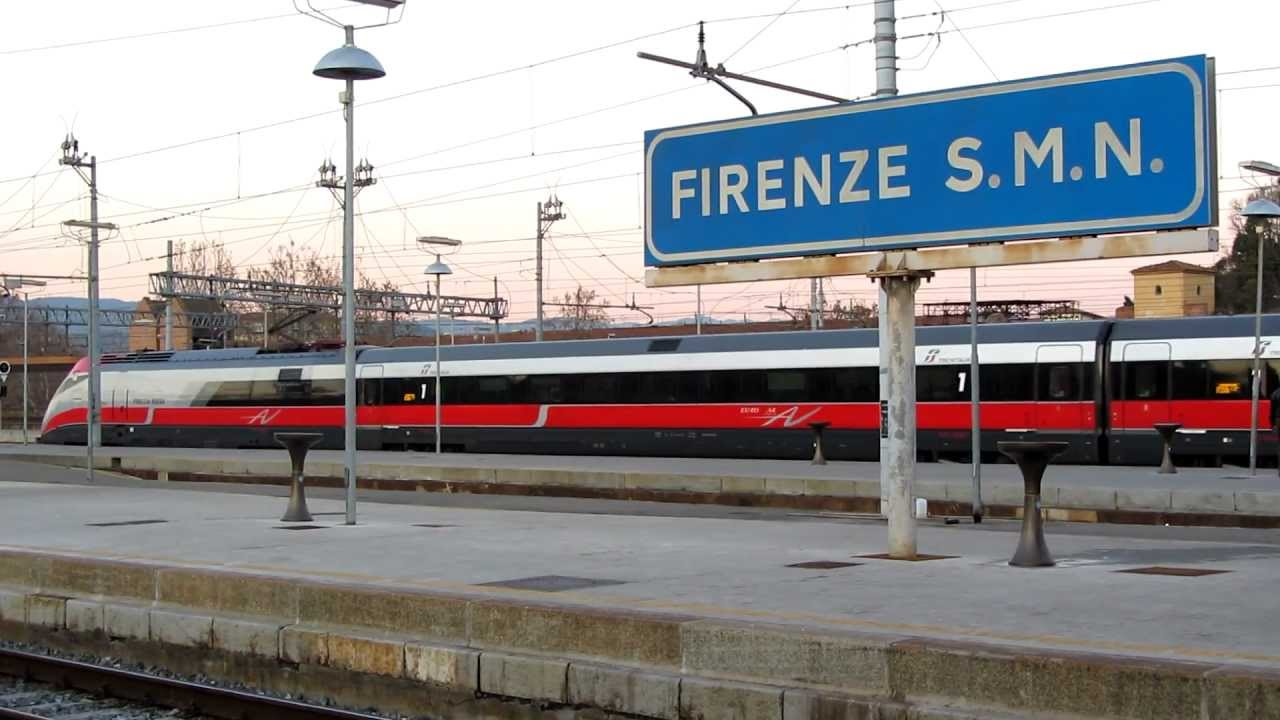
\includegraphics[width=0.7\linewidth]{img/frecciarossa}
	\caption{Treno in arrivo alla stazione ferroviaria di Firenze Santa Maria Novella}
	\label{fig:frecciarossa}
\end{figure}
Il trasporto ferrotramviario, di contro, vede l'utilizzo di treni dalle ridotte dimensioni, pi\'u leggeri di quelli usati nei sistemi ferroviari, e che hanno lo scopo di rappresentare un'alternativa per il cittadino all'utilizzo di mezzi privati durante i suoi spostamenti all'interno di un'area metropolitana. Quest'ultima caratteristica implica che l'ambiente operativo di un sistema ferrotramviario sia radicalmente diverso da quello di un sistema ferroviario: i treni si muovono lungo rotaie installate su strade urbane, quindi il traffico ferrotramviario \`e fuso con il traffico automobilistico, motociclistico, ciclistico e pedonale che caratterizza l'ambiente urbano, come mostrato nelle figure \ref{fig:danhai} e \ref{fig:tramschema}.\\*
\begin{figure}[h]
	\centering
	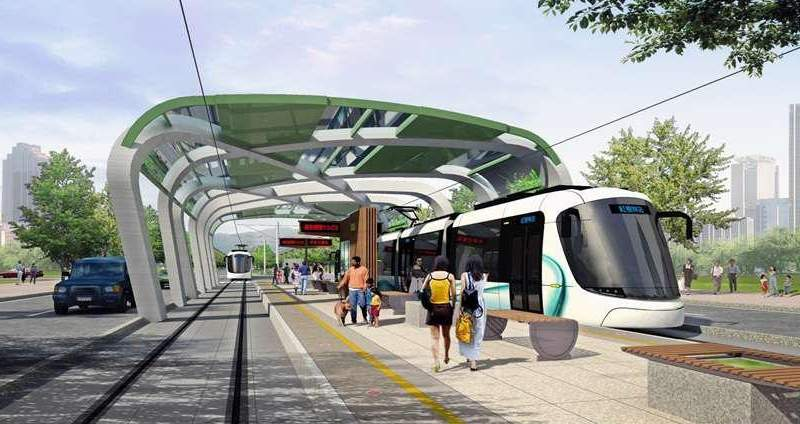
\includegraphics[width=0.7\linewidth]{img/danhai}
	\caption{Tramvia di Danhai, Taipan}
	\label{fig:danhai}
\end{figure}
\begin{figure}[h]
	\centering
	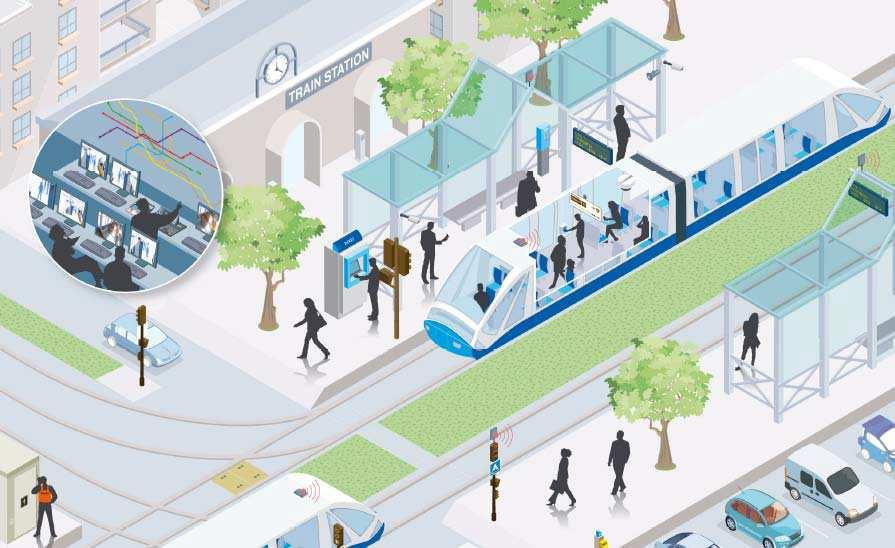
\includegraphics[width=0.7\linewidth]{img/twschema}
	\caption{Schema di un tipico scenario tramviario}
	\label{fig:tramschema}
\end{figure}
\section{Il Problema del Posizionamento}
Per posizionamento ferroviario, si intende la stima della posizione di un particolare treno all'interno di una particolare traccia ferroviaria. Spesso questa stima viene espressa come progressiva chilometrica rispetto all'origine della linea, oppure pi\'u raramente come coordinata geografica.\\*
Il problema del posizionamento sorge nel momento in cui, per ragioni di \emph{safety}, particolari sezioni di una traccia ferroviaria o ferrotramviaria, hanno caratteristiche tali da poter permettere il transito di un solo veicolo alla volta, come nel caso di una sezione di binario condivisa fra due opposti sensi di marcia, in cui la presenza di un unico veicolo \`e fondamentale per evitare impatti catastrofici.\\*Ogni qualvolta la \emph{safety} di un sistema risulti fondamentale, si parla di \emph{sistema critico} o \emph{safety-critical}.\\*
Gli odierni sistemi di posizionamento sono sistemi \emph{safety-critical} e si basano principalmente sull'utilizzo di strumenti installati a terra, che hanno lo scopo di rilevare il passaggio di un treno, e quindi di interagire con il sistema di \emph{interlocking} della traccia al fine di garantire, con un elevato livello di confidenza, un transito sicuro dei mezzi.\\*
Per elevato livello di confidenza si intendono rigorose evidenze matematiche sulla \emph{safety} del sistema di posizionamento.\\*Per quanto concerne la \emph{safety} in ambito ferroviario e ferrotramviario, esiste uno standard internazionale, il \emph{Safety Integrity Level (SIL)}. Esso si articola su cinque livelli, da \texttt{SIL-0} a \texttt{SIL-4}, ed un sistema, per essere \texttt{SIL-n}, con $0\le n\le 4$, deve disporre di documentate garanzie quantitative e qualitative circa il suo \emph{Mean Time to Failure (MTTF)}, ossia il tempo medio al fallimento, e sulle conseguenze di un suo eventuale fallimento.\\*
I sistemi ferroviari e ferrotramviari, per loro natura, sono sistemi cosiddetti \emph{fail-safe}, i quali si distinguono dai sistemi \emph{fail-operational} in quanto i primi devono poter essere in grado di fallire in modo sicuro, ad esempio un treno che si ferma in campagna non provocher\`a disastri ma solamente disagi ai passeggeri; ed i secondi devono invece garantire un livello minimo di operativit\`a anche in caso di fallimenti.\\*\`E esempio di un sistema \emph{fail-operational} un aereo che ha subito un fallimento e deve effettuare un atterragio di emergenza.
\subsubsection{Odierne Tecniche di Posizionamento}
I sistemi di posizionamento attualmente in uso sono basati su un'architettura distribuita composta dai seguenti blocchi:
\begin{itemize}
	\item Sottosistema di \emph{interlocking};
	\item Sottosistema di comunicazione \texttt{treno-traccia};
	\item Sottosistema semaforico.
\end{itemize}
Il sottosistema di \emph{interlocking} \`e la parte che si fa effettivamente carico di offrire al treno un attraversamento sicuro di una \emph{Junction Area (JA)}, ossia del confine tra una sezione non-critica e una sezione critica di una traccia.\\*
Un sistema di \emph{interlocking} \`e composto dai seguenti elementi:
\begin{itemize}
	\item \emph{Switch Control Unit (UCS)}:\\*
	Piattaforma certificata \texttt{SIL-3} che rappresenta il nucleo del sistema di \emph{interlocking} e che implementa l'intera logica di gestione di una JA. Un UCS dispone di un'interfaccia di \emph{Input/Output} (I/O) verso gli elementi di \emph{interlocking} installati a terra che ne consente un controllo sicuro in accordo allo standard \texttt{SIL-3}.
\begin{figure}[h]
		\centering
		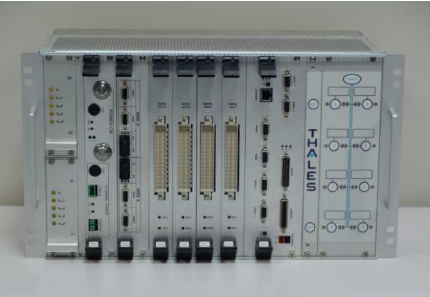
\includegraphics[width=0.7\linewidth]{img/ucs}
		\caption{UCS realizzato da Thales Italia SPA}
		\label{fig:ucs}
\end{figure}
	\item Conta Assi:\\*
	Il Conta Assi, o in inglese \emph{Axle Counter} (AC), \`e un sistema certificato \texttt{SIL-3} che ha lo scopo di rilevare la presenza del treno e fornire quindi lo stato di occupazione della sezione di traccia in cui l'AC \`e installato.
\begin{figure}[h]
	\centering
	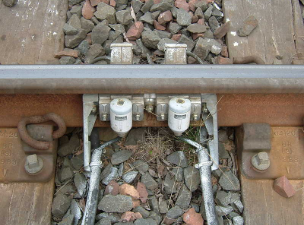
\includegraphics[width=11cm,height=3.1cm]{img/axlecounter}
	\caption{Conta Assi}
	\label{fig:ac}
\end{figure}
	\item \emph{Point Machines}:\\*
	Le \emph{Point Machines} infine, sono degli strmvumenti certificati \texttt{SIL-3} che hanno lo scopo di direzionare le rotaie verso una determinata sezione di traccia.
	\begin{figure}[h]
		\centering
		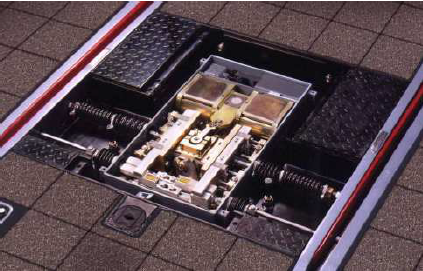
\includegraphics[width=0.7\linewidth]{img/pointmachine}
		\caption{Esempio di \emph{Point Machine} installata su una traccia ferrotramviaria}
		\label{fig:pointmachine}
	\end{figure}
\end{itemize}
Il sottosistema di comunicazione treno-traccia \`e gestito da un computer installato bordo treno, ed ha lo scopo di fornire funzionalit\`a non legate alla \emph{safety} e pertanto poco interessanti. Questo sistema viene principalmente utilizzato per monitorare lo stato del traffico ferrotramviario in una architettura di \emph{monitoring} centralizzata e si basa su comunicazioni \emph{wireless}. In alcune applicazioni pu\'o comprendere una comunicazione pi\'u o meno diretta con il sistema di \emph{interlocking} allo scopo di segnalare l'avvicinamento del treno a una JA.\\*
Il sottosistema semaforico prende in ingresso informazioni dal sistema di \emph{interlocking} ed eventualmente, dal sistema di comunicazione treno-traccia, e gestisce i segnali luminosi da mostrare sui semafori a un macchinista che si appresta a superare una JA.\\*In tabella \ref{tab:sem} viene riportata la lista dei segnali semaforici utilizzati nel contesto ferrotramviario.
\begin{table}
\begin{tabular}{|c|c|c|}
	\hline 
	\textbf{Segnale} & \textbf{Descrizione} & \textbf{Significato} \\

	\hline
	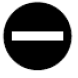
\includegraphics{img/stopsemaphore}& Barra bianca orizzontale & Fermarsi \\ 
	\hline 
	
\includegraphics{img/gosemaphore}& Barra bianca verticale  & Procedere avanti \\ 
	\hline 
	
\includegraphics{img/rightsemaphore}& Barra bianca ruotata di 45 gradi & Procedere solo a destra \\ 
	\hline 
	
\includegraphics{img/leftsemaphore}& Barra bianca ruotata di -45 gradi & Procedere solo a sinistra \\ 
	\hline 
\end{tabular} 
\caption{Segnalazioni semaforiche ferrotramviarie}
\label{tab:sem}
\end{table}
\subsection{Possibili Sviluppi}
Le attuali tecniche di posizionamento richiedono un intervento trascurabile di computer installati a bordo e una grande quantit\`a di apparati installati a terra. Mentre i computer di bordo si fanno carico principalmente della comunicazione treno-traccia e forniscono in generale funzionalit\`a non legate alla \emph{safety}, gli apparati installati a terra sono costosi e hanno un impatto ambientale non trascurabile.\\*
\`E possibile invece considerare il treno e il computer di bordo come un unico sistema, ossia il treno viene modellato come un vero e proprio \emph{Cyber-Physical System}.\\*
Un \emph{Cyber-Physical System} (CPS) \`e un sistema composto da una parte \emph{fisica} e da una parte \emph{cyber}. Il sottosistema fisico \`e composto da sensori e attuatori che hanno rispettivamente lo scopo di rilevare lo stato dell'ambiente circostante e di alterarlo se necessario. Il sottosistema \emph{cyber} \`e un vero e proprio elaboratore, che dispone di processore e memoria, e delle interfaccie di I/O verso i sensori e gli attuatori. Una simile architettura di sistema, rende possibile sfruttare le capacit\`a di calcolo dei moderni processori per implementare algoritmi anche molto complessi per il \emph{processing} di grandi quantit\`a di dati provenienti dai sensori.\\*
Lo scopo della Tesi \`e quello di mostrare come pu\`o un CPS sostituire il complesso e costoso sistema di posizionamento tuttora operante, attraverso l'uso combinato di un insieme di sensori i cui dati rilevati vengono processati da un algoritmo noto come \emph{Sensor Fusion Algorithm} (SFA).\\*
\begin{figure}[h]
	\centering
	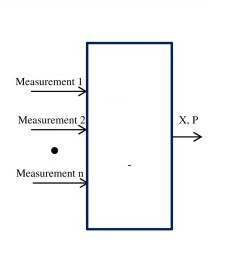
\includegraphics{img/sfaschema}
	\caption{Schema SFA}
	\label{fig:sfa}
\end{figure}
\\*
Tale algoritmo \`e schematizzabile come una \emph{black-box} la quale, ricevuti i dati dei sensori in ingresso, fornisce in uscita la posizione del treno lungo la traccia ferroviaria (figura \ref{fig:sfa}).\\*
Utilizzando SFA, il treno \`e in grado di auto-posizionarsi, capacit\`a che minimizza la necessit\`a di installare apparati di terra.\\*
La necessit\`a di utilizzare un algoritmo che tenga conto delle misurazioni di un \emph{set} di sensori, in luogo di un semplice \emph{processing} di insiemi di singole misure provenienti dalla stessa sorgente, risiede nella capacit\`a che ha SFA di \emph{correggere} il rumore che disturba le singole misurazioni, realizzando cos\`i una nuova misura pi\`u accurata di quella che si avrebbe considerando i sensori come sorgenti distinte.\\*

